\documentclass[11pt]{article}
\usepackage[textwidth=18.0cm, textheight=23.0cm, top=2.0cm]{geometry}
\usepackage{pst-all}
\usepackage{amssymb}
\usepackage{tikz}
\usepackage{underscore}\begin{document}
\pagestyle{empty}


ClassName: \underline{\textbf{Class_03.2bp-20}}
\par
BinSize: \underline{\textbf{40 × 40}}
\par
ReduceSize: \underline{\textbf{40 × 40}}
\par
TypeNum: \underline{\textbf{59}}
\par
Num: \underline{\textbf{60}}
\par
OutS: \underline{\textbf{25600}}
\par
InS: \underline{\textbf{21567}}
\par
Rate: \underline{\textbf{0.842}}
\par
UB: \underline{\textbf{16}}
\par
LB0: \underline{\textbf{16}}
\par
LB: \underline{\textbf{16}}
\par
LBWithCut: \underline{\textbf{16}}
\par
NodeCut: \underline{\textbf{0}}
\par
ExtendedNodeCnt: \underline{\textbf{1}}
\par
GenNodeCnt: \underline{\textbf{1}}
\par
PrimalNode: \underline{\textbf{0}}
\par
ColumnCount: \underline{\textbf{16}}
\par
TotalCutCount: \underline{\textbf{0}}
\par
RootCutCount: \underline{\textbf{0}}
\par
LPSolverCnt: \underline{\textbf{1}}
\par
PricingSolverCnt: \underline{\textbf{0}}
\par
BranchAndBoundNum: \underline{\textbf{1}}
\par
isOpt: \underline{\textbf{true}}
\par
TimeOnInitSolution: \underline{\textbf{0.080 s}}
\par
TimeOnPrimal: \underline{\textbf{0.000 s}}
\par
TimeOnPricing: \underline{\textbf{0.000 s}}
\par
TimeOnRmp: \underline{\textbf{0.078 s}}
\par
TotalTime: \underline{\textbf{0.221 s}}
\par
\newpage


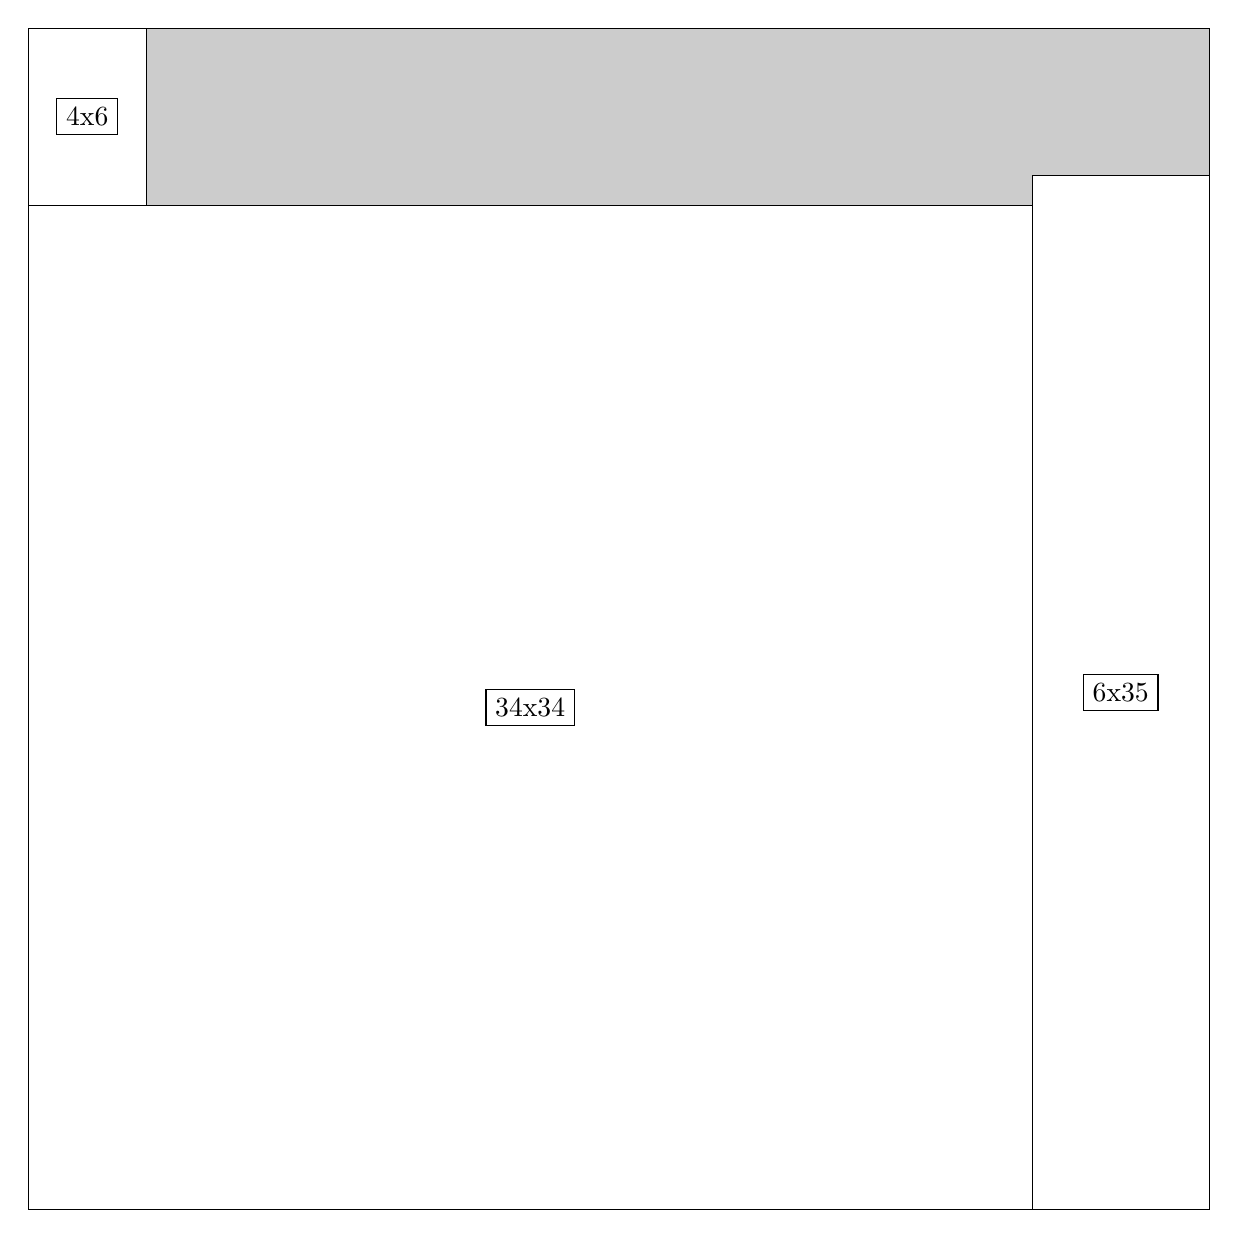
\begin{tikzpicture}[shorten >=1pt,scale=1.0,every node/.style={scale=1.0},->]
\tikzstyle{vertex}=[circle,fill=black!25,minimum size=14pt,inner sep=0pt]
\filldraw[fill=gray!40!white, draw=black] (0,0) rectangle (15.0,15.0);
\foreach \name/\x/\y/\w/\h in {34x34/0.0/0.0/12.75/12.75,6x35/12.75/0.0/2.25/13.125,4x6/0.0/12.75/1.5/2.25}
\filldraw[fill=white!40!white, draw=black] (\x,\y) rectangle node[draw] (\name) {\name} ++(\w,\h);
\end{tikzpicture}


w =34 , h =34 , x =0 , y =0 , v =1156
\par
w =6 , h =35 , x =34 , y =0 , v =210
\par
w =4 , h =6 , x =0 , y =34 , v =24
\par
\newpage


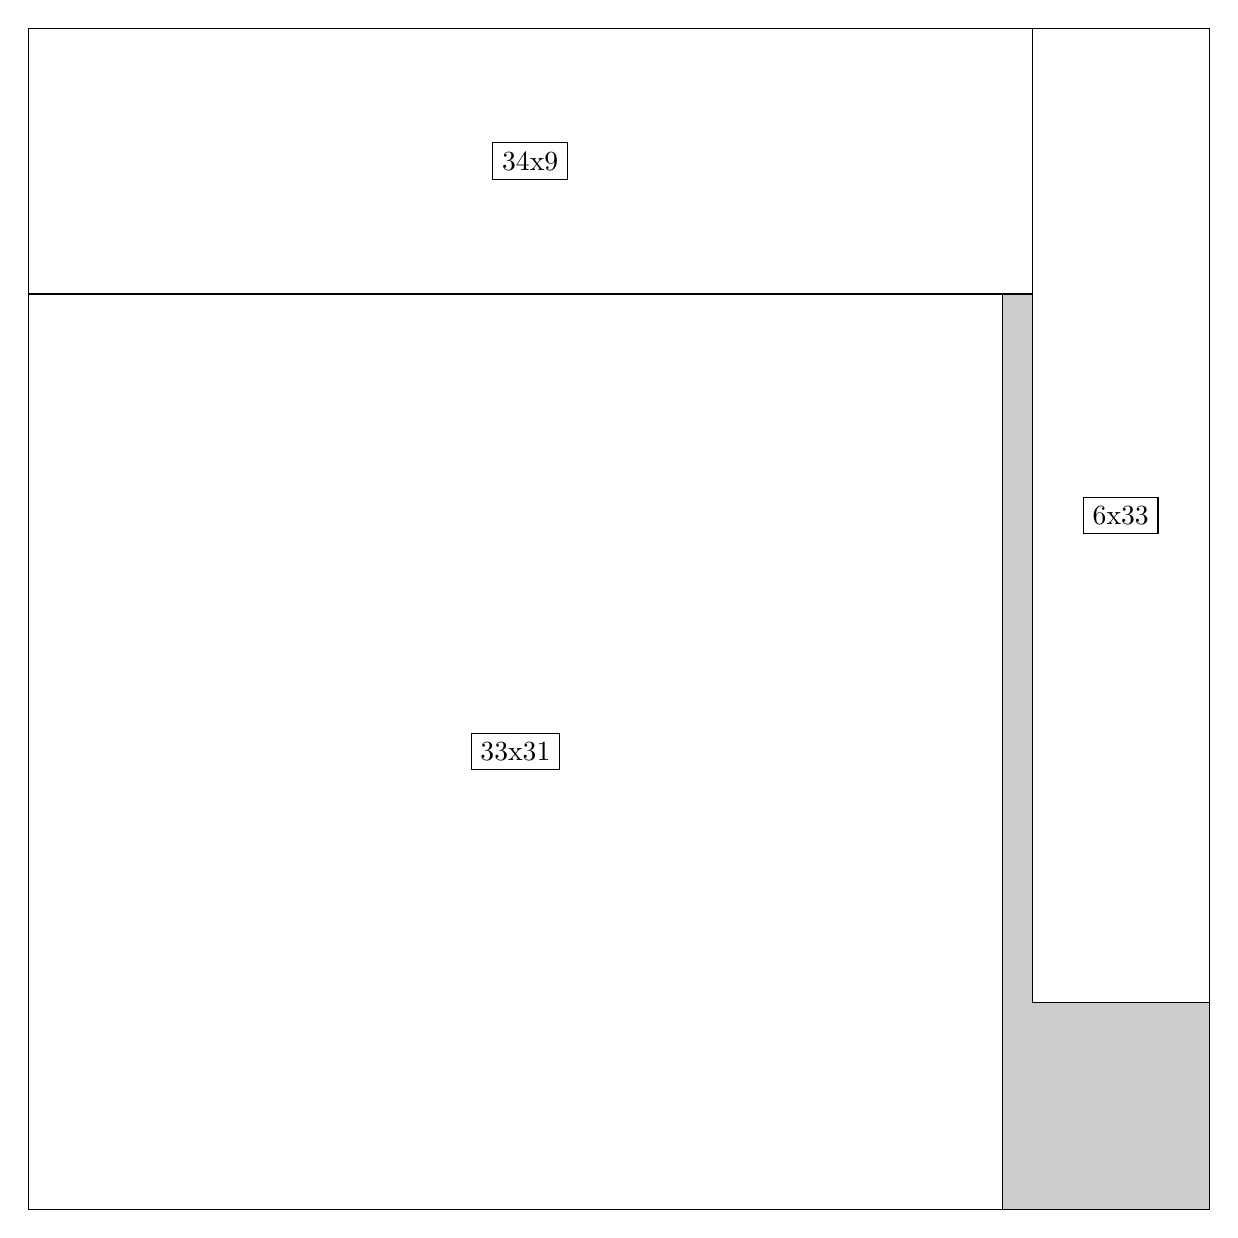
\begin{tikzpicture}[shorten >=1pt,scale=1.0,every node/.style={scale=1.0},->]
\tikzstyle{vertex}=[circle,fill=black!25,minimum size=14pt,inner sep=0pt]
\filldraw[fill=gray!40!white, draw=black] (0,0) rectangle (15.0,15.0);
\foreach \name/\x/\y/\w/\h in {33x31/0.0/0.0/12.375/11.625,34x9/0.0/11.625/12.75/3.375,6x33/12.75/2.625/2.25/12.375}
\filldraw[fill=white!40!white, draw=black] (\x,\y) rectangle node[draw] (\name) {\name} ++(\w,\h);
\end{tikzpicture}


w =33 , h =31 , x =0 , y =0 , v =1023
\par
w =34 , h =9 , x =0 , y =31 , v =306
\par
w =6 , h =33 , x =34 , y =7 , v =198
\par
\newpage


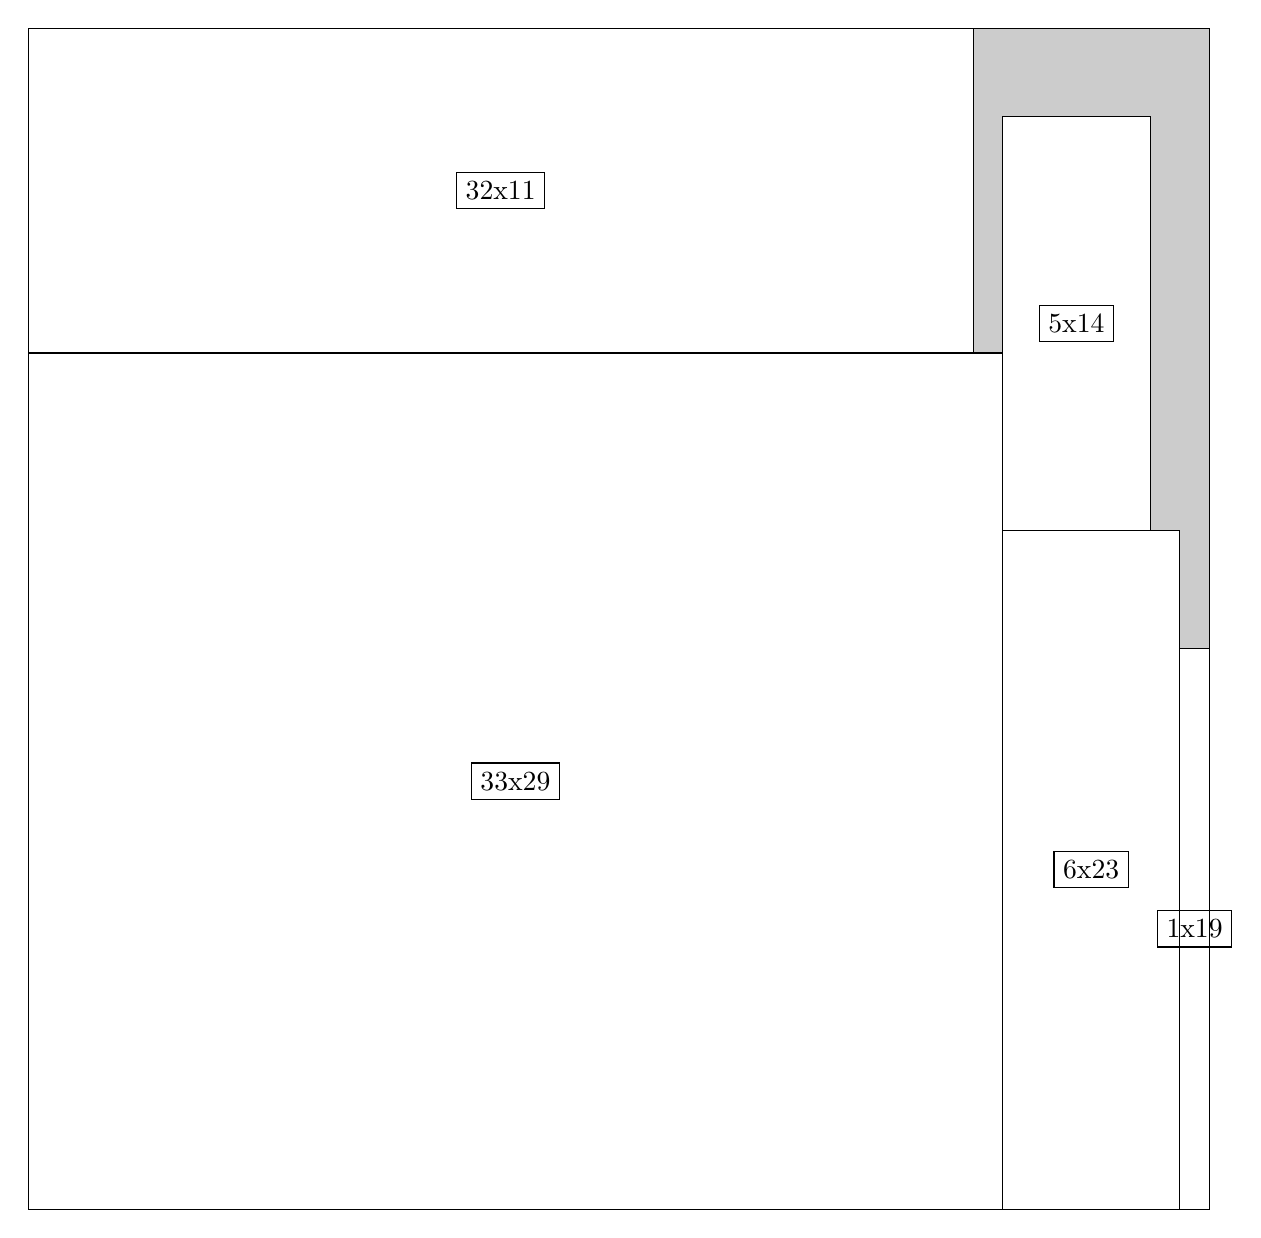
\begin{tikzpicture}[shorten >=1pt,scale=1.0,every node/.style={scale=1.0},->]
\tikzstyle{vertex}=[circle,fill=black!25,minimum size=14pt,inner sep=0pt]
\filldraw[fill=gray!40!white, draw=black] (0,0) rectangle (15.0,15.0);
\foreach \name/\x/\y/\w/\h in {33x29/0.0/0.0/12.375/10.875,32x11/0.0/10.875/12.0/4.125,6x23/12.375/0.0/2.25/8.625,5x14/12.375/8.625/1.875/5.25,1x19/14.625/0.0/0.375/7.125}
\filldraw[fill=white!40!white, draw=black] (\x,\y) rectangle node[draw] (\name) {\name} ++(\w,\h);
\end{tikzpicture}


w =33 , h =29 , x =0 , y =0 , v =957
\par
w =32 , h =11 , x =0 , y =29 , v =352
\par
w =6 , h =23 , x =33 , y =0 , v =138
\par
w =5 , h =14 , x =33 , y =23 , v =70
\par
w =1 , h =19 , x =39 , y =0 , v =19
\par
\newpage


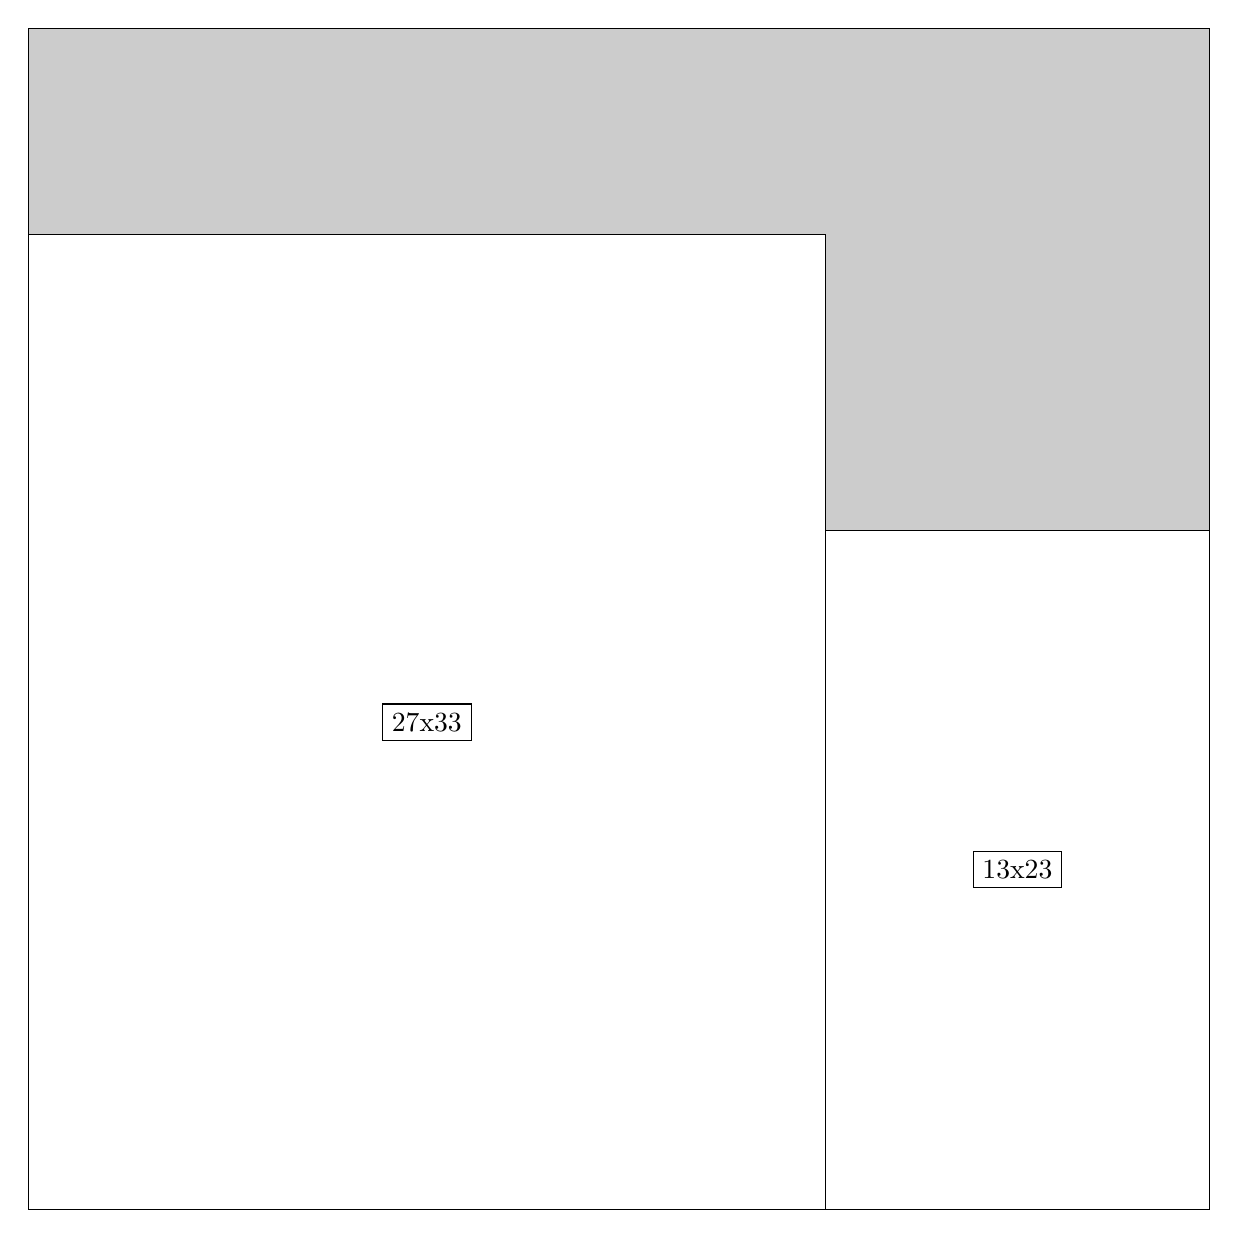
\begin{tikzpicture}[shorten >=1pt,scale=1.0,every node/.style={scale=1.0},->]
\tikzstyle{vertex}=[circle,fill=black!25,minimum size=14pt,inner sep=0pt]
\filldraw[fill=gray!40!white, draw=black] (0,0) rectangle (15.0,15.0);
\foreach \name/\x/\y/\w/\h in {27x33/0.0/0.0/10.125/12.375,13x23/10.125/0.0/4.875/8.625}
\filldraw[fill=white!40!white, draw=black] (\x,\y) rectangle node[draw] (\name) {\name} ++(\w,\h);
\end{tikzpicture}


w =27 , h =33 , x =0 , y =0 , v =891
\par
w =13 , h =23 , x =27 , y =0 , v =299
\par
\newpage


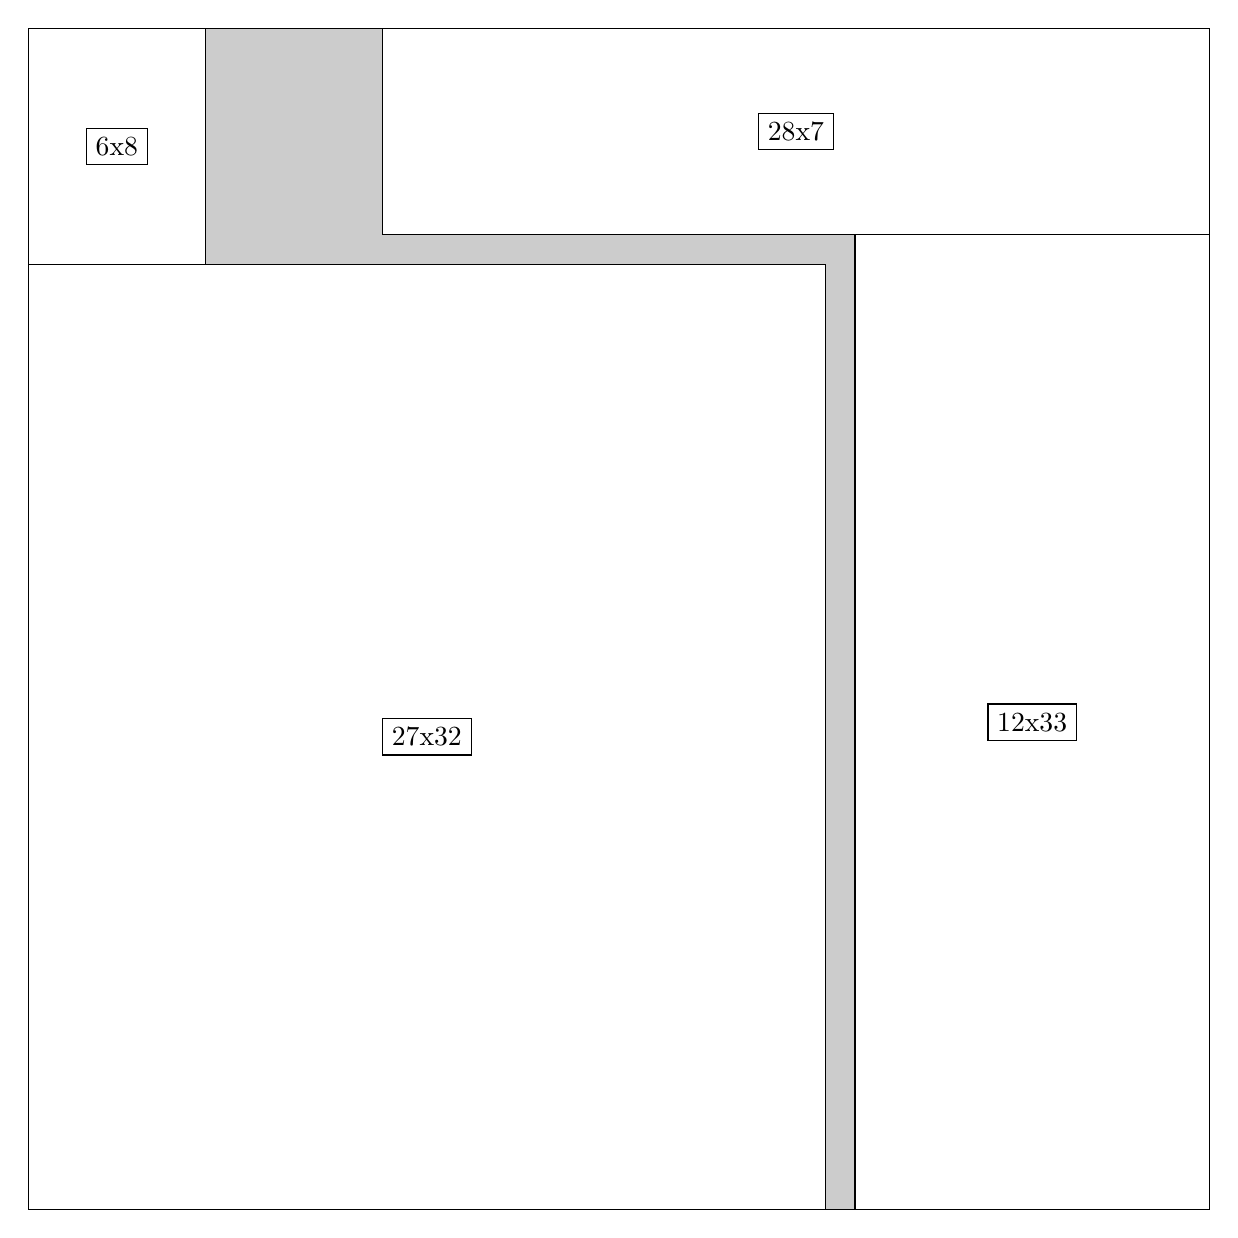
\begin{tikzpicture}[shorten >=1pt,scale=1.0,every node/.style={scale=1.0},->]
\tikzstyle{vertex}=[circle,fill=black!25,minimum size=14pt,inner sep=0pt]
\filldraw[fill=gray!40!white, draw=black] (0,0) rectangle (15.0,15.0);
\foreach \name/\x/\y/\w/\h in {27x32/0.0/0.0/10.125/12.0,12x33/10.5/0.0/4.5/12.375,28x7/4.5/12.375/10.5/2.625,6x8/0.0/12.0/2.25/3.0}
\filldraw[fill=white!40!white, draw=black] (\x,\y) rectangle node[draw] (\name) {\name} ++(\w,\h);
\end{tikzpicture}


w =27 , h =32 , x =0 , y =0 , v =864
\par
w =12 , h =33 , x =28 , y =0 , v =396
\par
w =28 , h =7 , x =12 , y =33 , v =196
\par
w =6 , h =8 , x =0 , y =32 , v =48
\par
\newpage


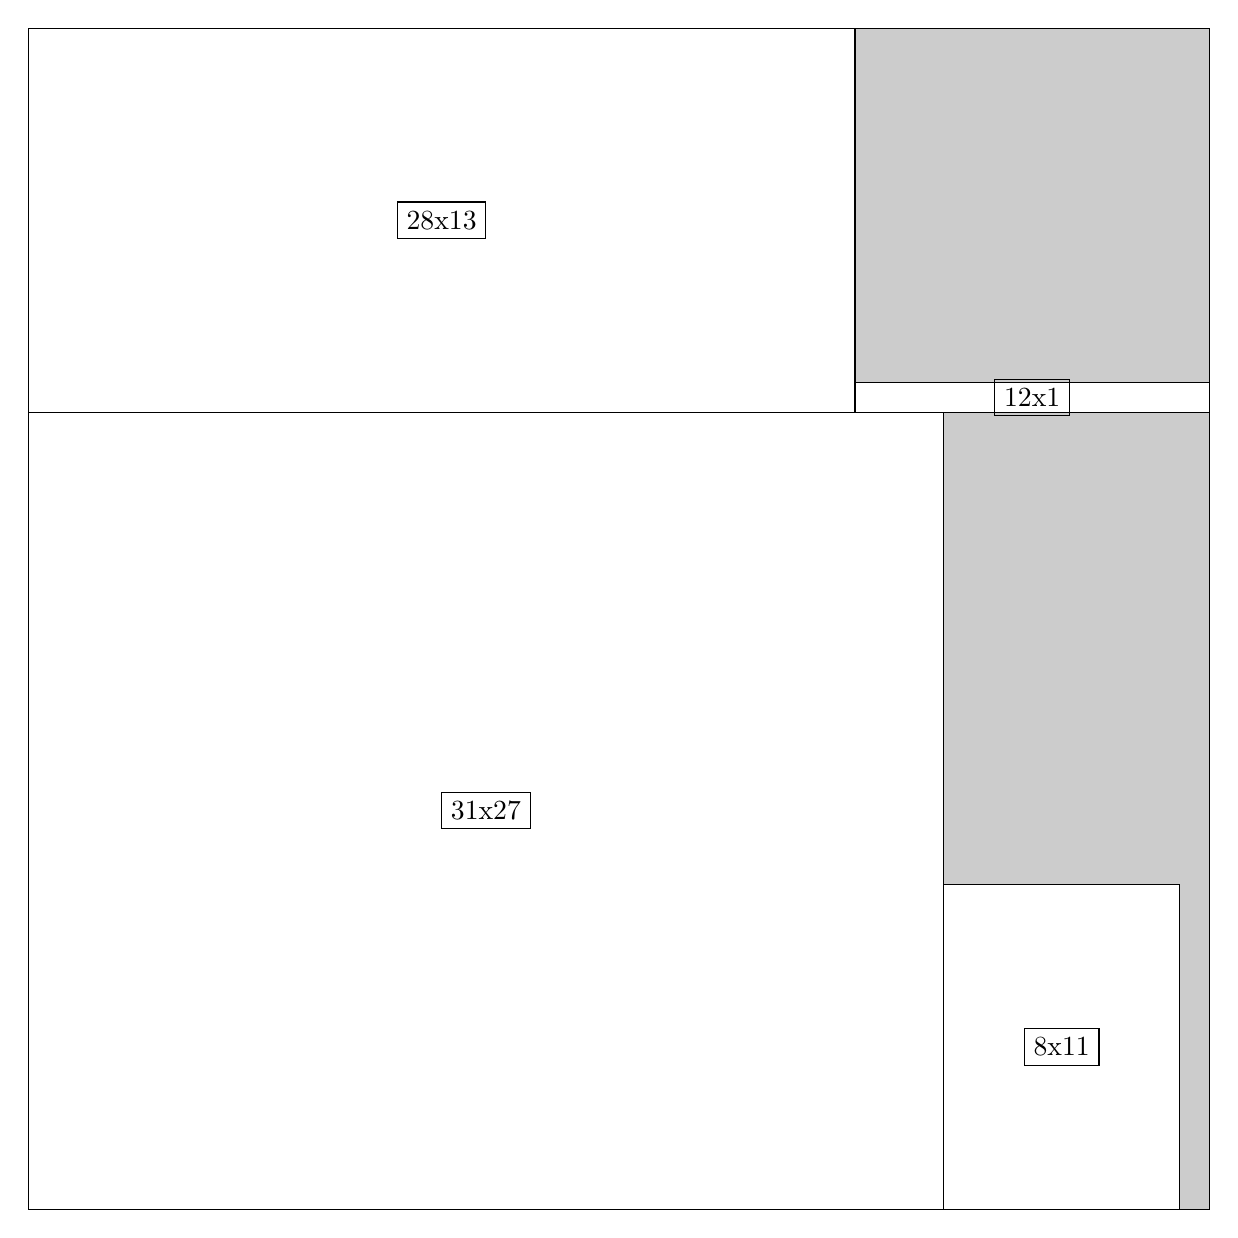
\begin{tikzpicture}[shorten >=1pt,scale=1.0,every node/.style={scale=1.0},->]
\tikzstyle{vertex}=[circle,fill=black!25,minimum size=14pt,inner sep=0pt]
\filldraw[fill=gray!40!white, draw=black] (0,0) rectangle (15.0,15.0);
\foreach \name/\x/\y/\w/\h in {31x27/0.0/0.0/11.625/10.125,28x13/0.0/10.125/10.5/4.875,8x11/11.625/0.0/3.0/4.125,12x1/10.5/10.125/4.5/0.375}
\filldraw[fill=white!40!white, draw=black] (\x,\y) rectangle node[draw] (\name) {\name} ++(\w,\h);
\end{tikzpicture}


w =31 , h =27 , x =0 , y =0 , v =837
\par
w =28 , h =13 , x =0 , y =27 , v =364
\par
w =8 , h =11 , x =31 , y =0 , v =88
\par
w =12 , h =1 , x =28 , y =27 , v =12
\par
\newpage


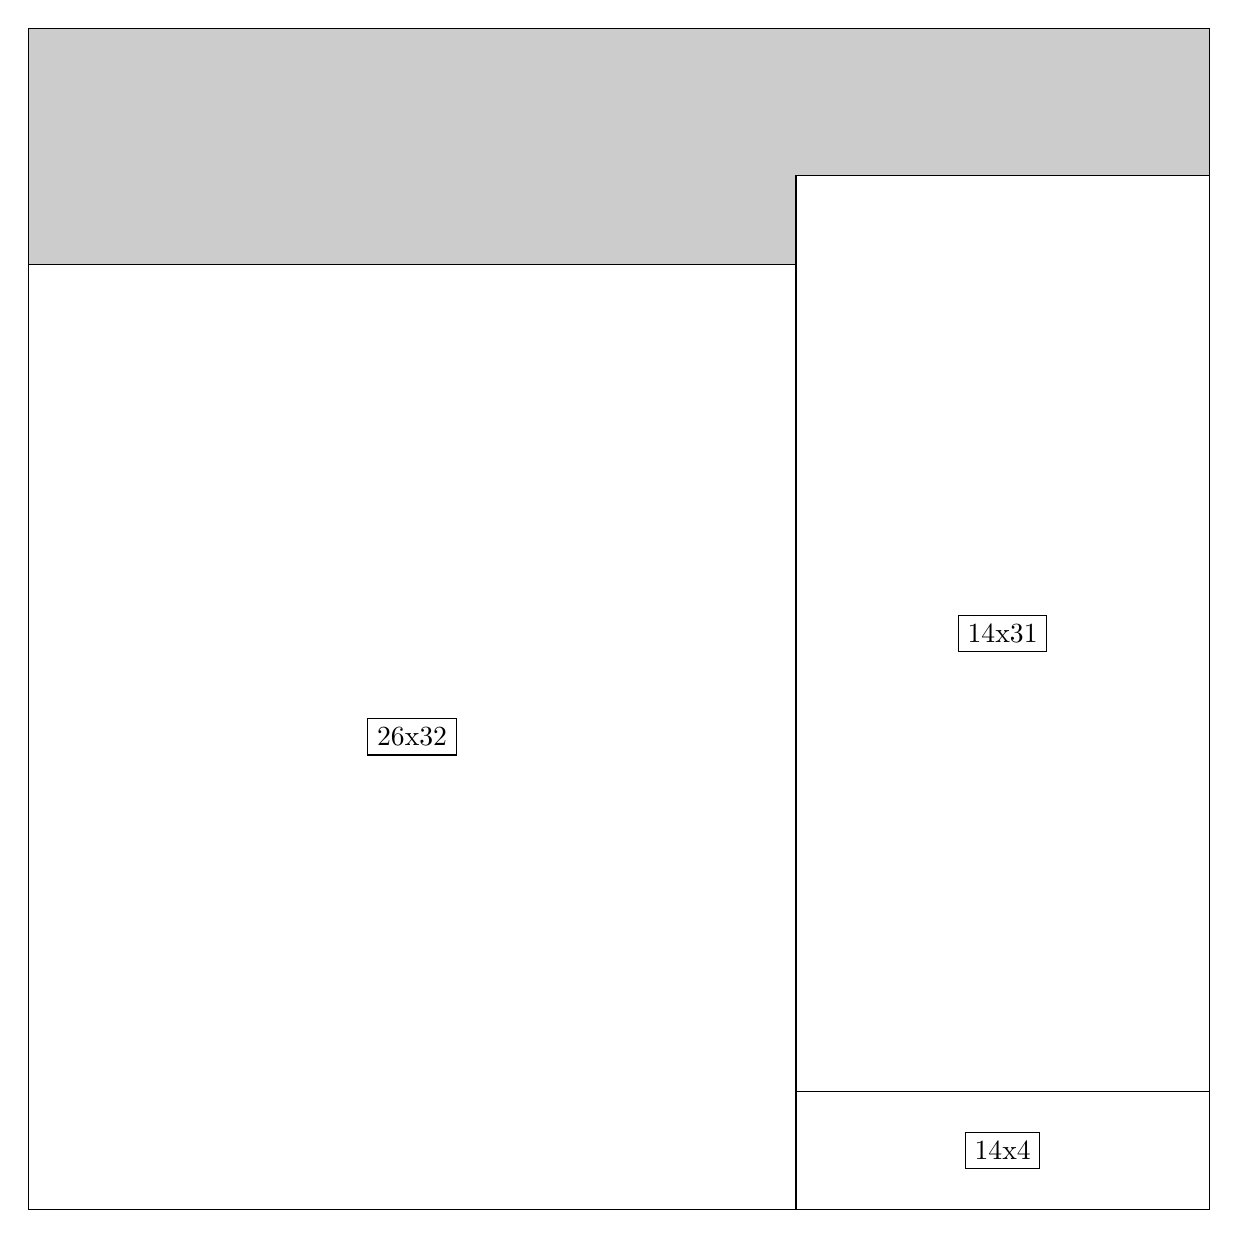
\begin{tikzpicture}[shorten >=1pt,scale=1.0,every node/.style={scale=1.0},->]
\tikzstyle{vertex}=[circle,fill=black!25,minimum size=14pt,inner sep=0pt]
\filldraw[fill=gray!40!white, draw=black] (0,0) rectangle (15.0,15.0);
\foreach \name/\x/\y/\w/\h in {26x32/0.0/0.0/9.75/12.0,14x31/9.75/1.5/5.25/11.625,14x4/9.75/0.0/5.25/1.5}
\filldraw[fill=white!40!white, draw=black] (\x,\y) rectangle node[draw] (\name) {\name} ++(\w,\h);
\end{tikzpicture}


w =26 , h =32 , x =0 , y =0 , v =832
\par
w =14 , h =31 , x =26 , y =4 , v =434
\par
w =14 , h =4 , x =26 , y =0 , v =56
\par
\newpage


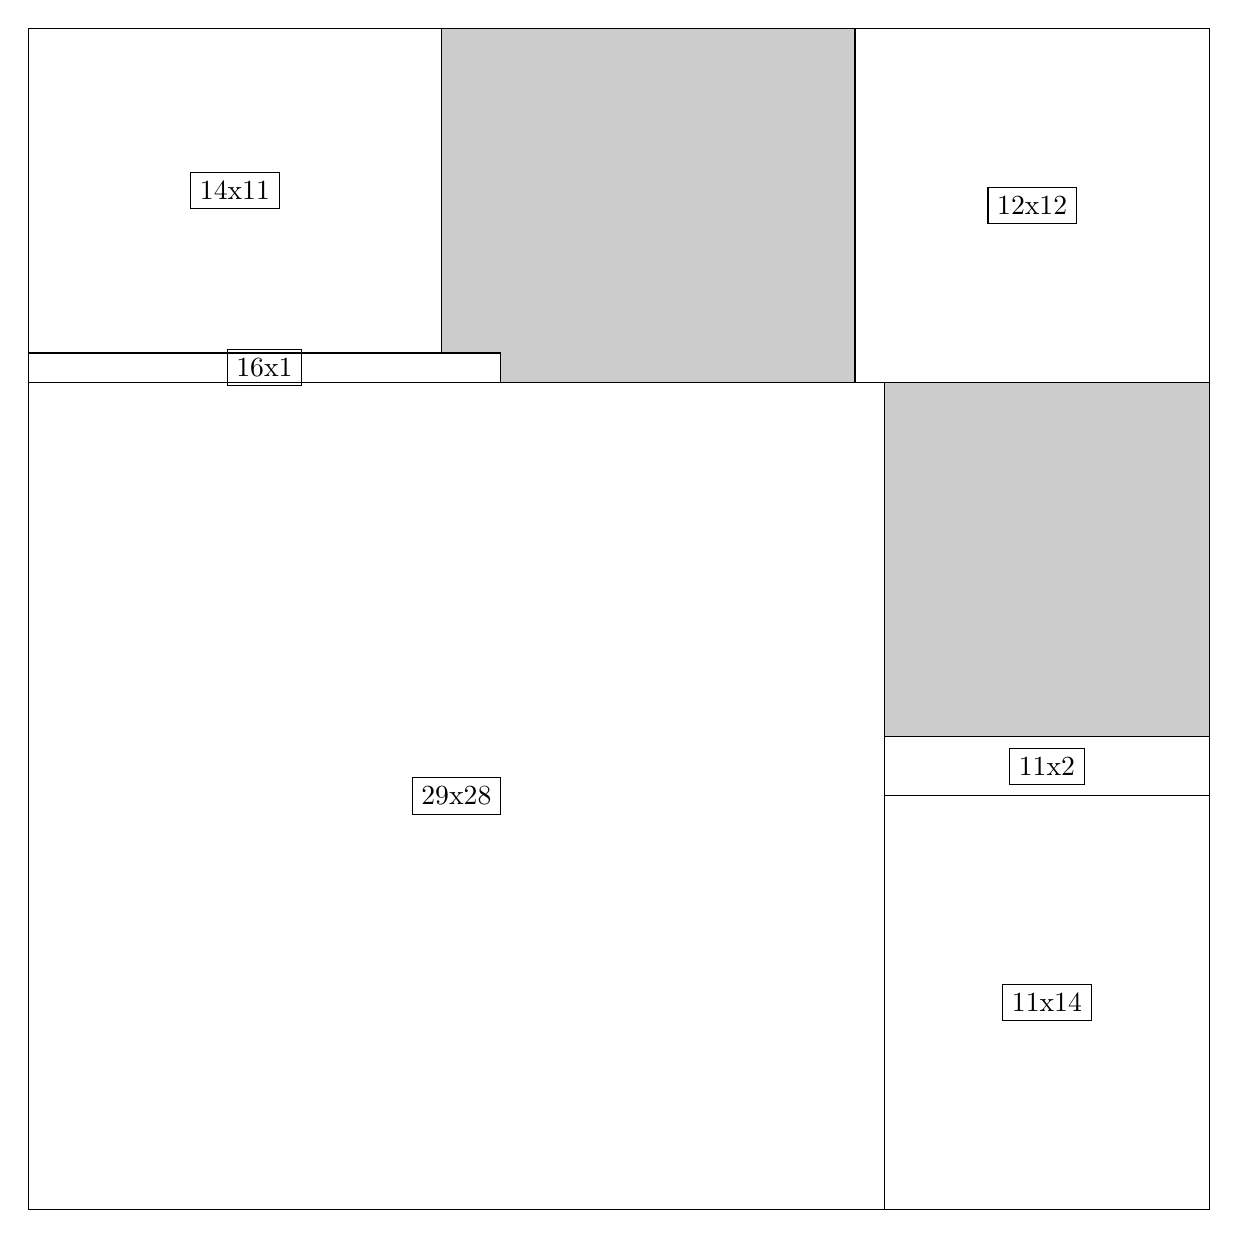
\begin{tikzpicture}[shorten >=1pt,scale=1.0,every node/.style={scale=1.0},->]
\tikzstyle{vertex}=[circle,fill=black!25,minimum size=14pt,inner sep=0pt]
\filldraw[fill=gray!40!white, draw=black] (0,0) rectangle (15.0,15.0);
\foreach \name/\x/\y/\w/\h in {29x28/0.0/0.0/10.875/10.5,14x11/0.0/10.875/5.25/4.125,11x14/10.875/0.0/4.125/5.25,12x12/10.5/10.5/4.5/4.5,11x2/10.875/5.25/4.125/0.75,16x1/0.0/10.5/6.0/0.375}
\filldraw[fill=white!40!white, draw=black] (\x,\y) rectangle node[draw] (\name) {\name} ++(\w,\h);
\end{tikzpicture}


w =29 , h =28 , x =0 , y =0 , v =812
\par
w =14 , h =11 , x =0 , y =29 , v =154
\par
w =11 , h =14 , x =29 , y =0 , v =154
\par
w =12 , h =12 , x =28 , y =28 , v =144
\par
w =11 , h =2 , x =29 , y =14 , v =22
\par
w =16 , h =1 , x =0 , y =28 , v =16
\par
\newpage


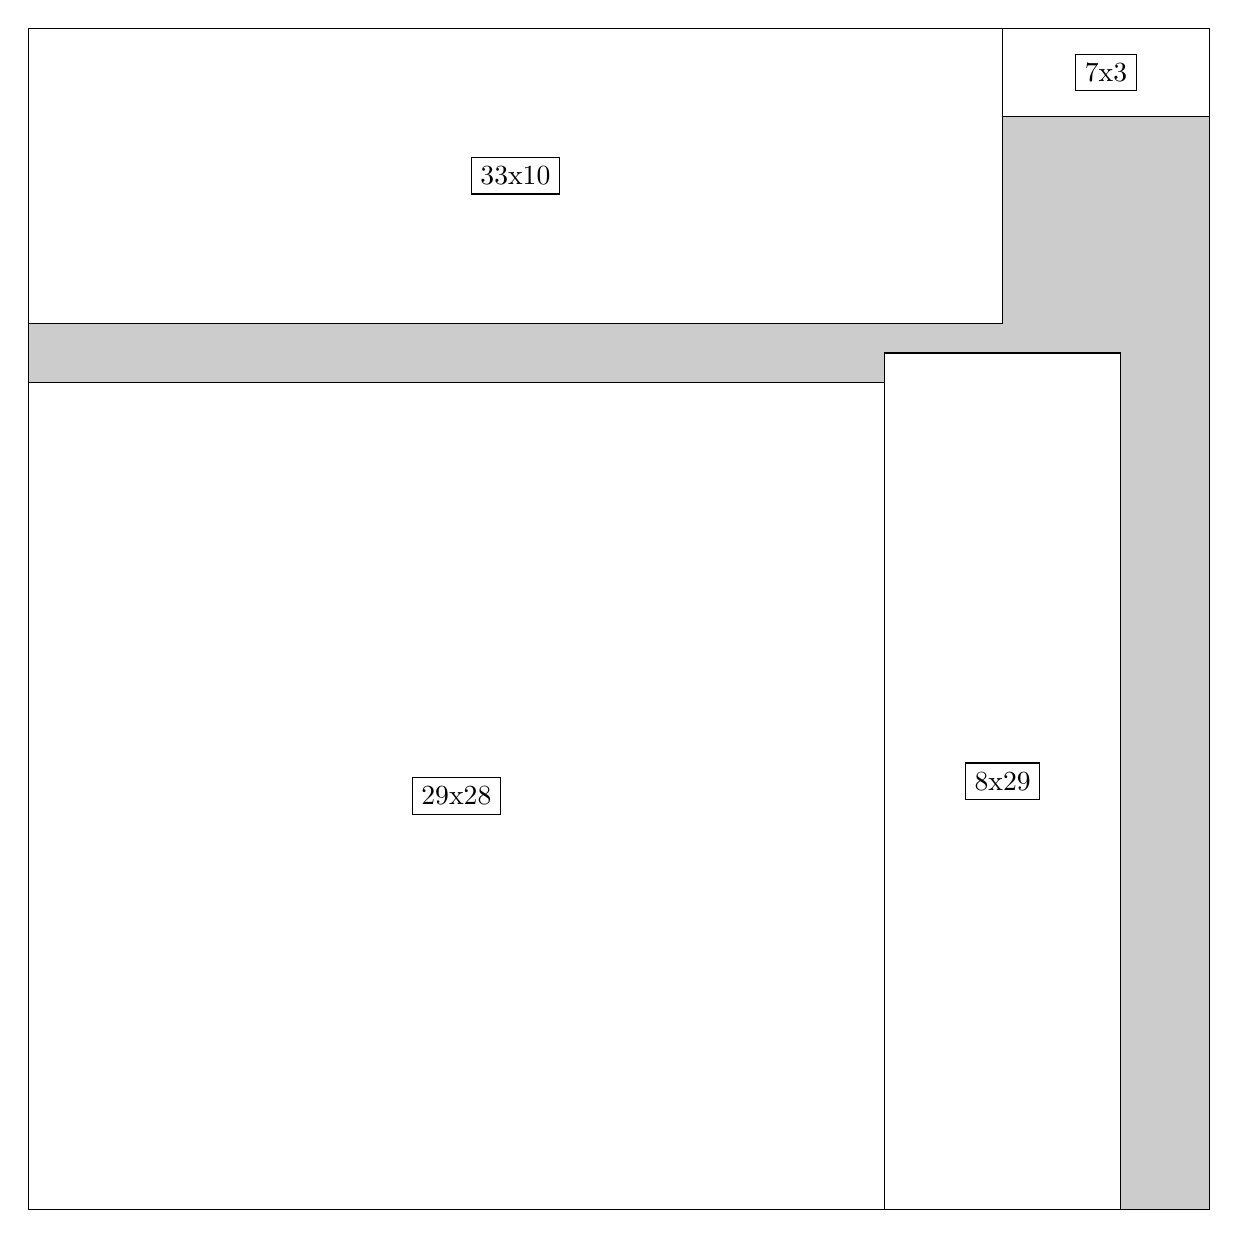
\begin{tikzpicture}[shorten >=1pt,scale=1.0,every node/.style={scale=1.0},->]
\tikzstyle{vertex}=[circle,fill=black!25,minimum size=14pt,inner sep=0pt]
\filldraw[fill=gray!40!white, draw=black] (0,0) rectangle (15.0,15.0);
\foreach \name/\x/\y/\w/\h in {29x28/0.0/0.0/10.875/10.5,33x10/0.0/11.25/12.375/3.75,8x29/10.875/0.0/3.0/10.875,7x3/12.375/13.875/2.625/1.125}
\filldraw[fill=white!40!white, draw=black] (\x,\y) rectangle node[draw] (\name) {\name} ++(\w,\h);
\end{tikzpicture}


w =29 , h =28 , x =0 , y =0 , v =812
\par
w =33 , h =10 , x =0 , y =30 , v =330
\par
w =8 , h =29 , x =29 , y =0 , v =232
\par
w =7 , h =3 , x =33 , y =37 , v =21
\par
\newpage


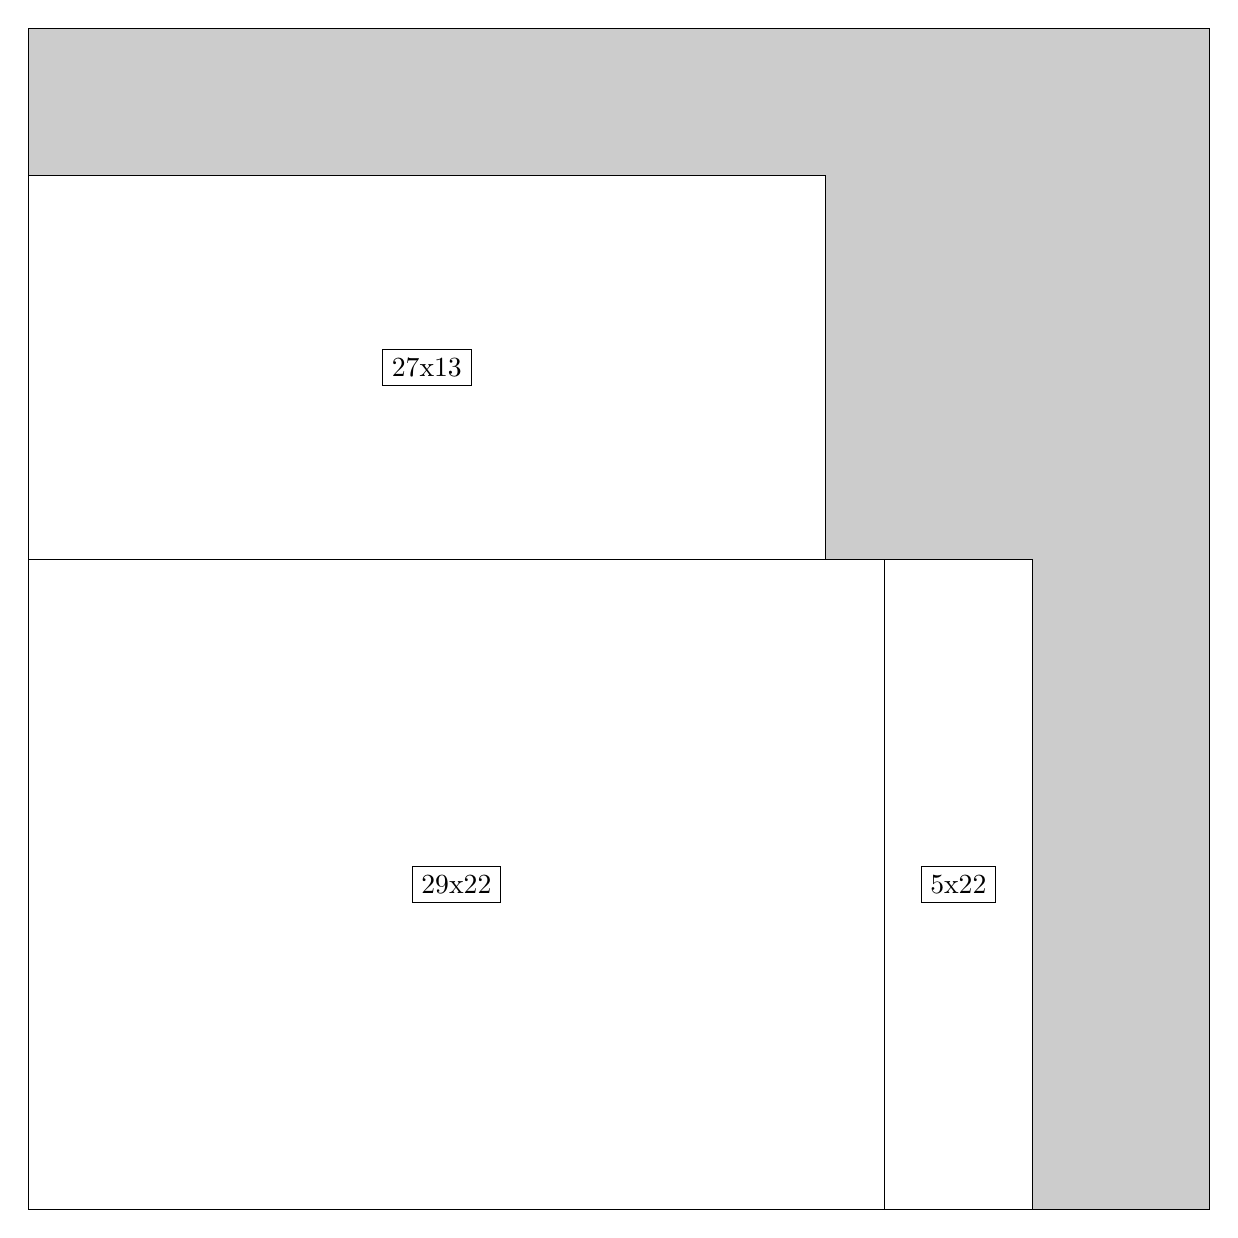
\begin{tikzpicture}[shorten >=1pt,scale=1.0,every node/.style={scale=1.0},->]
\tikzstyle{vertex}=[circle,fill=black!25,minimum size=14pt,inner sep=0pt]
\filldraw[fill=gray!40!white, draw=black] (0,0) rectangle (15.0,15.0);
\foreach \name/\x/\y/\w/\h in {29x22/0.0/0.0/10.875/8.25,27x13/0.0/8.25/10.125/4.875,5x22/10.875/0.0/1.875/8.25}
\filldraw[fill=white!40!white, draw=black] (\x,\y) rectangle node[draw] (\name) {\name} ++(\w,\h);
\end{tikzpicture}


w =29 , h =22 , x =0 , y =0 , v =638
\par
w =27 , h =13 , x =0 , y =22 , v =351
\par
w =5 , h =22 , x =29 , y =0 , v =110
\par
\newpage


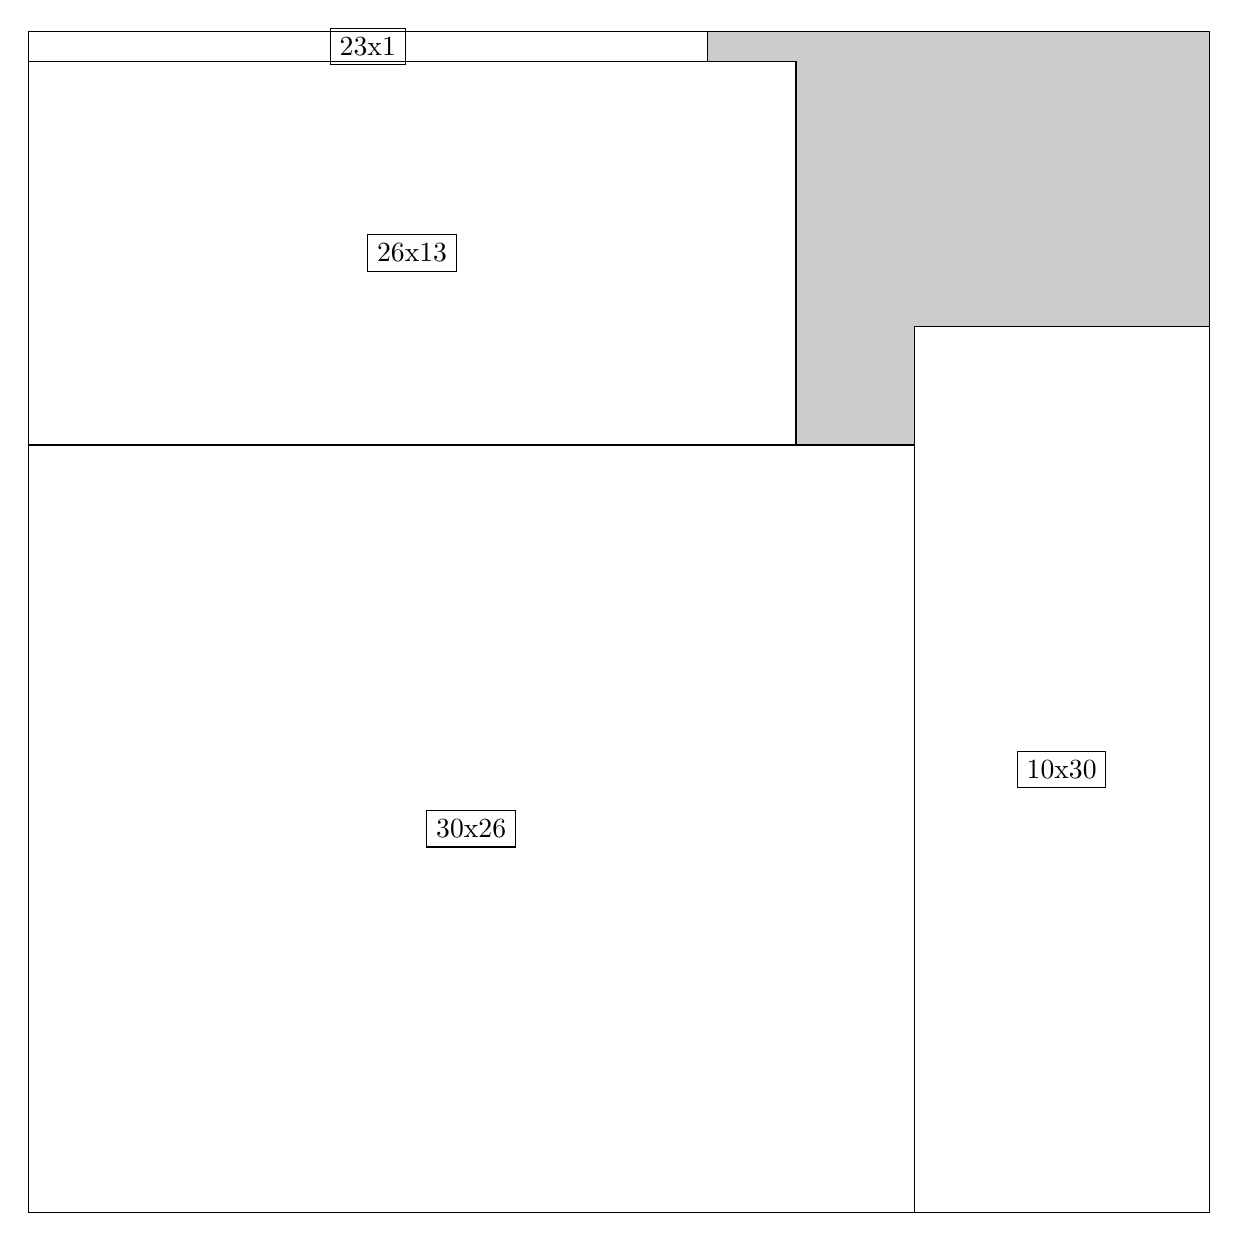
\begin{tikzpicture}[shorten >=1pt,scale=1.0,every node/.style={scale=1.0},->]
\tikzstyle{vertex}=[circle,fill=black!25,minimum size=14pt,inner sep=0pt]
\filldraw[fill=gray!40!white, draw=black] (0,0) rectangle (15.0,15.0);
\foreach \name/\x/\y/\w/\h in {30x26/0.0/0.0/11.25/9.75,26x13/0.0/9.75/9.75/4.875,10x30/11.25/0.0/3.75/11.25,23x1/0.0/14.625/8.625/0.375}
\filldraw[fill=white!40!white, draw=black] (\x,\y) rectangle node[draw] (\name) {\name} ++(\w,\h);
\end{tikzpicture}


w =30 , h =26 , x =0 , y =0 , v =780
\par
w =26 , h =13 , x =0 , y =26 , v =338
\par
w =10 , h =30 , x =30 , y =0 , v =300
\par
w =23 , h =1 , x =0 , y =39 , v =23
\par
\newpage


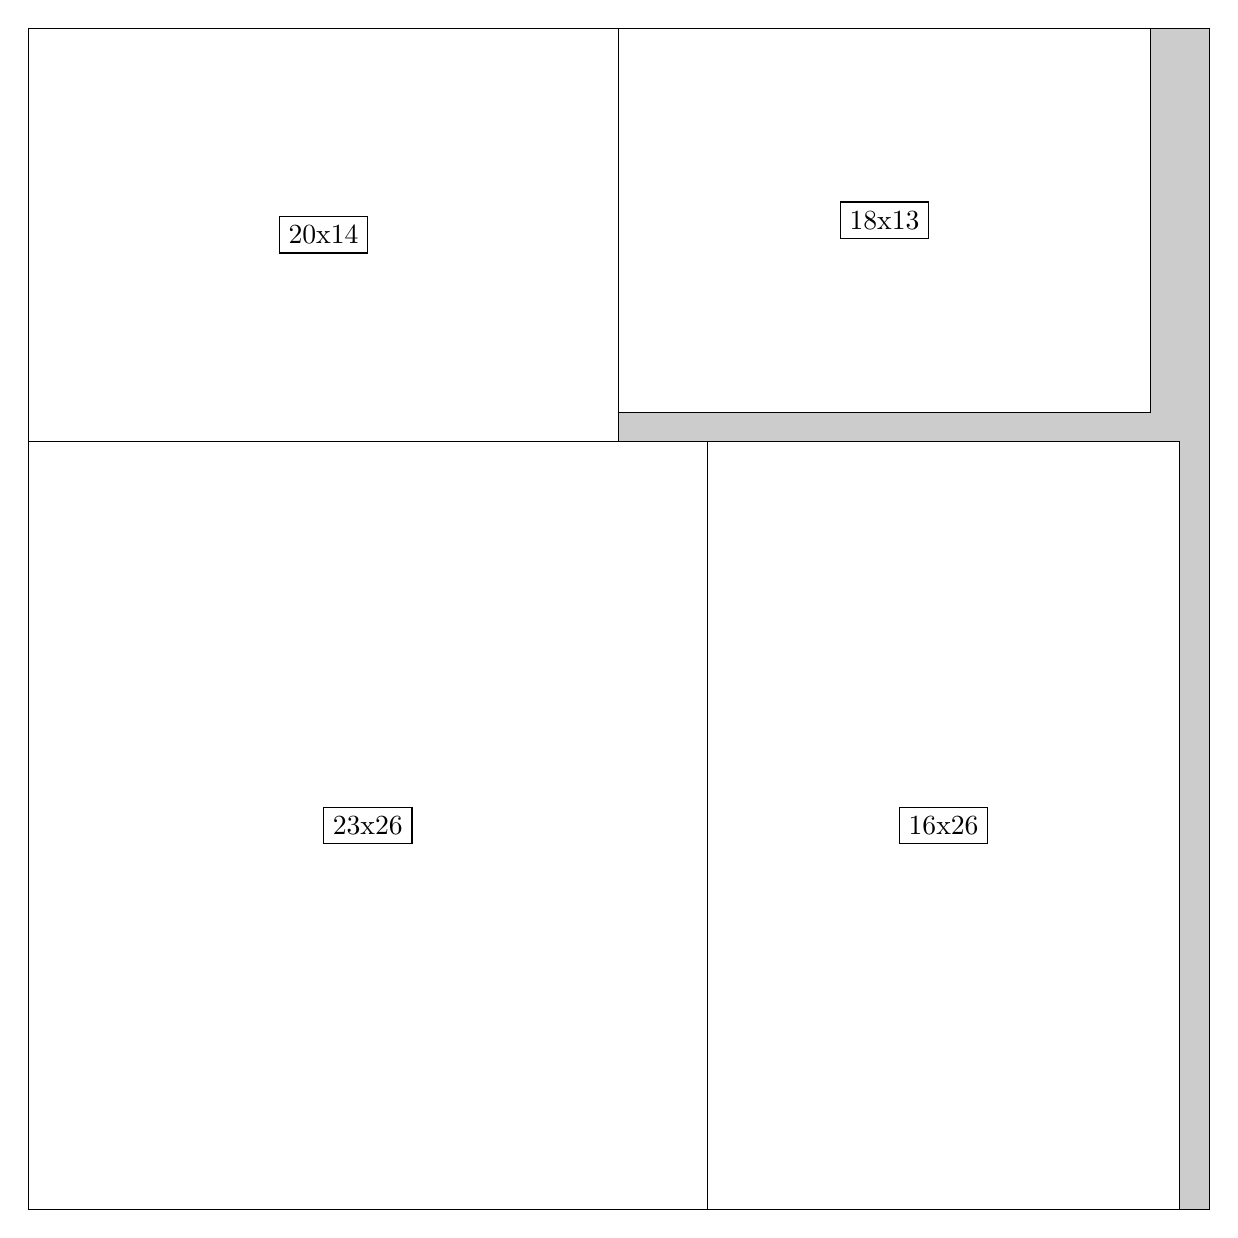
\begin{tikzpicture}[shorten >=1pt,scale=1.0,every node/.style={scale=1.0},->]
\tikzstyle{vertex}=[circle,fill=black!25,minimum size=14pt,inner sep=0pt]
\filldraw[fill=gray!40!white, draw=black] (0,0) rectangle (15.0,15.0);
\foreach \name/\x/\y/\w/\h in {23x26/0.0/0.0/8.625/9.75,16x26/8.625/0.0/6.0/9.75,20x14/0.0/9.75/7.5/5.25,18x13/7.5/10.125/6.75/4.875}
\filldraw[fill=white!40!white, draw=black] (\x,\y) rectangle node[draw] (\name) {\name} ++(\w,\h);
\end{tikzpicture}


w =23 , h =26 , x =0 , y =0 , v =598
\par
w =16 , h =26 , x =23 , y =0 , v =416
\par
w =20 , h =14 , x =0 , y =26 , v =280
\par
w =18 , h =13 , x =20 , y =27 , v =234
\par
\newpage


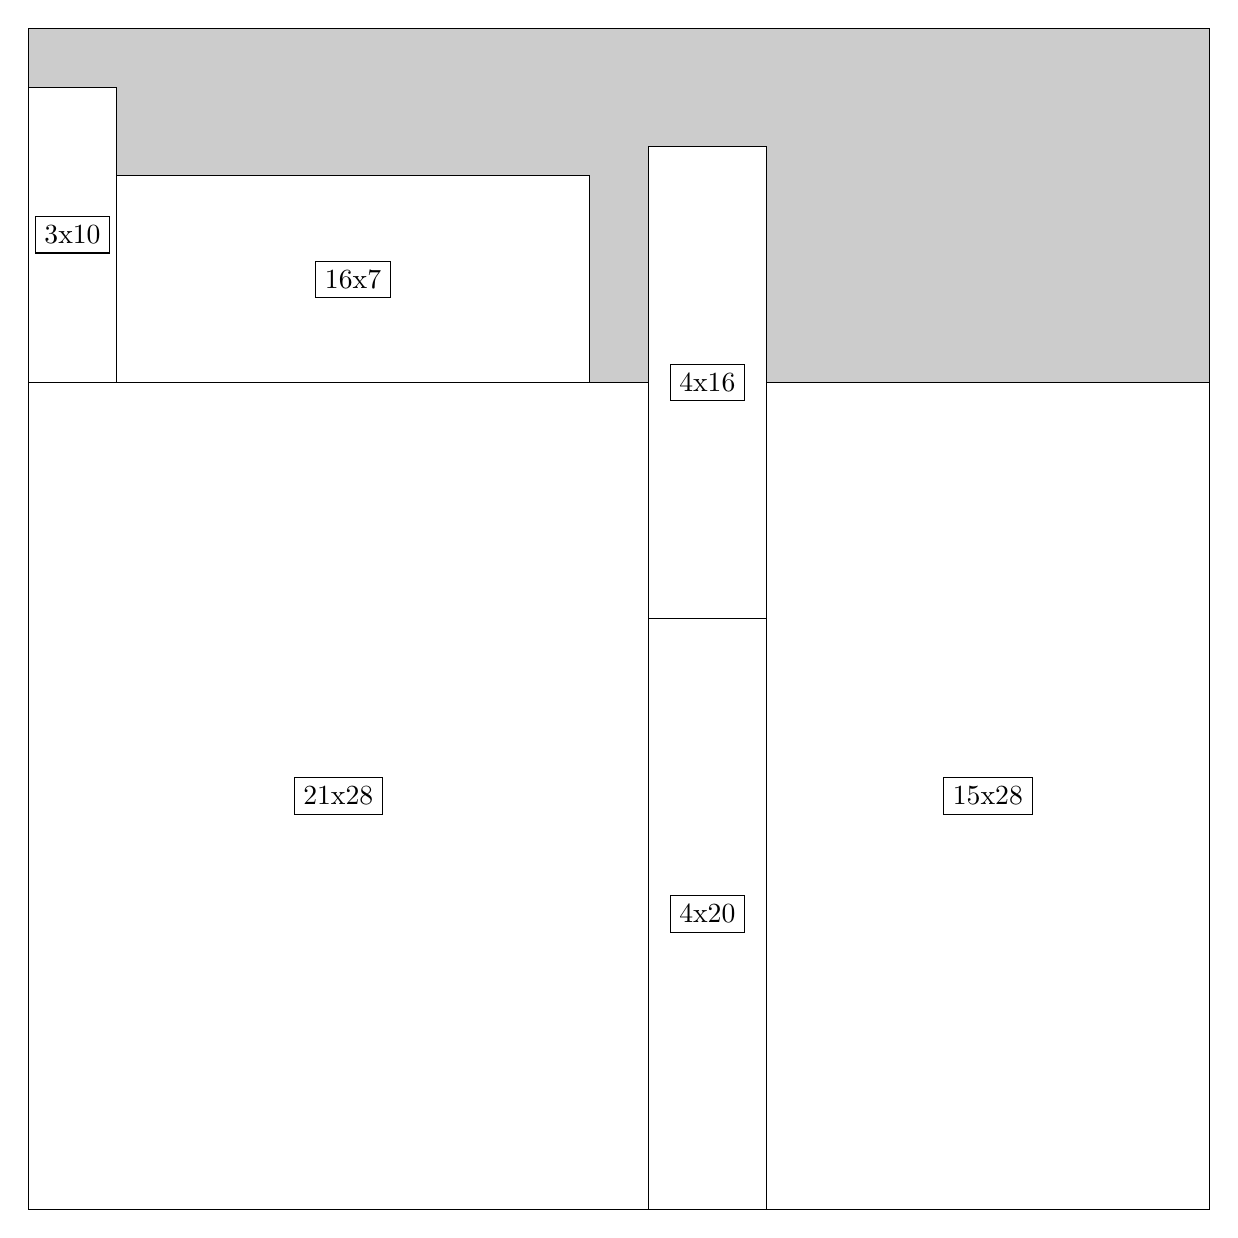
\begin{tikzpicture}[shorten >=1pt,scale=1.0,every node/.style={scale=1.0},->]
\tikzstyle{vertex}=[circle,fill=black!25,minimum size=14pt,inner sep=0pt]
\filldraw[fill=gray!40!white, draw=black] (0,0) rectangle (15.0,15.0);
\foreach \name/\x/\y/\w/\h in {21x28/0.0/0.0/7.875/10.5,15x28/9.375/0.0/5.625/10.5,16x7/1.125/10.5/6.0/2.625,4x20/7.875/0.0/1.5/7.5,4x16/7.875/7.5/1.5/6.0,3x10/0.0/10.5/1.125/3.75}
\filldraw[fill=white!40!white, draw=black] (\x,\y) rectangle node[draw] (\name) {\name} ++(\w,\h);
\end{tikzpicture}


w =21 , h =28 , x =0 , y =0 , v =588
\par
w =15 , h =28 , x =25 , y =0 , v =420
\par
w =16 , h =7 , x =3 , y =28 , v =112
\par
w =4 , h =20 , x =21 , y =0 , v =80
\par
w =4 , h =16 , x =21 , y =20 , v =64
\par
w =3 , h =10 , x =0 , y =28 , v =30
\par
\newpage


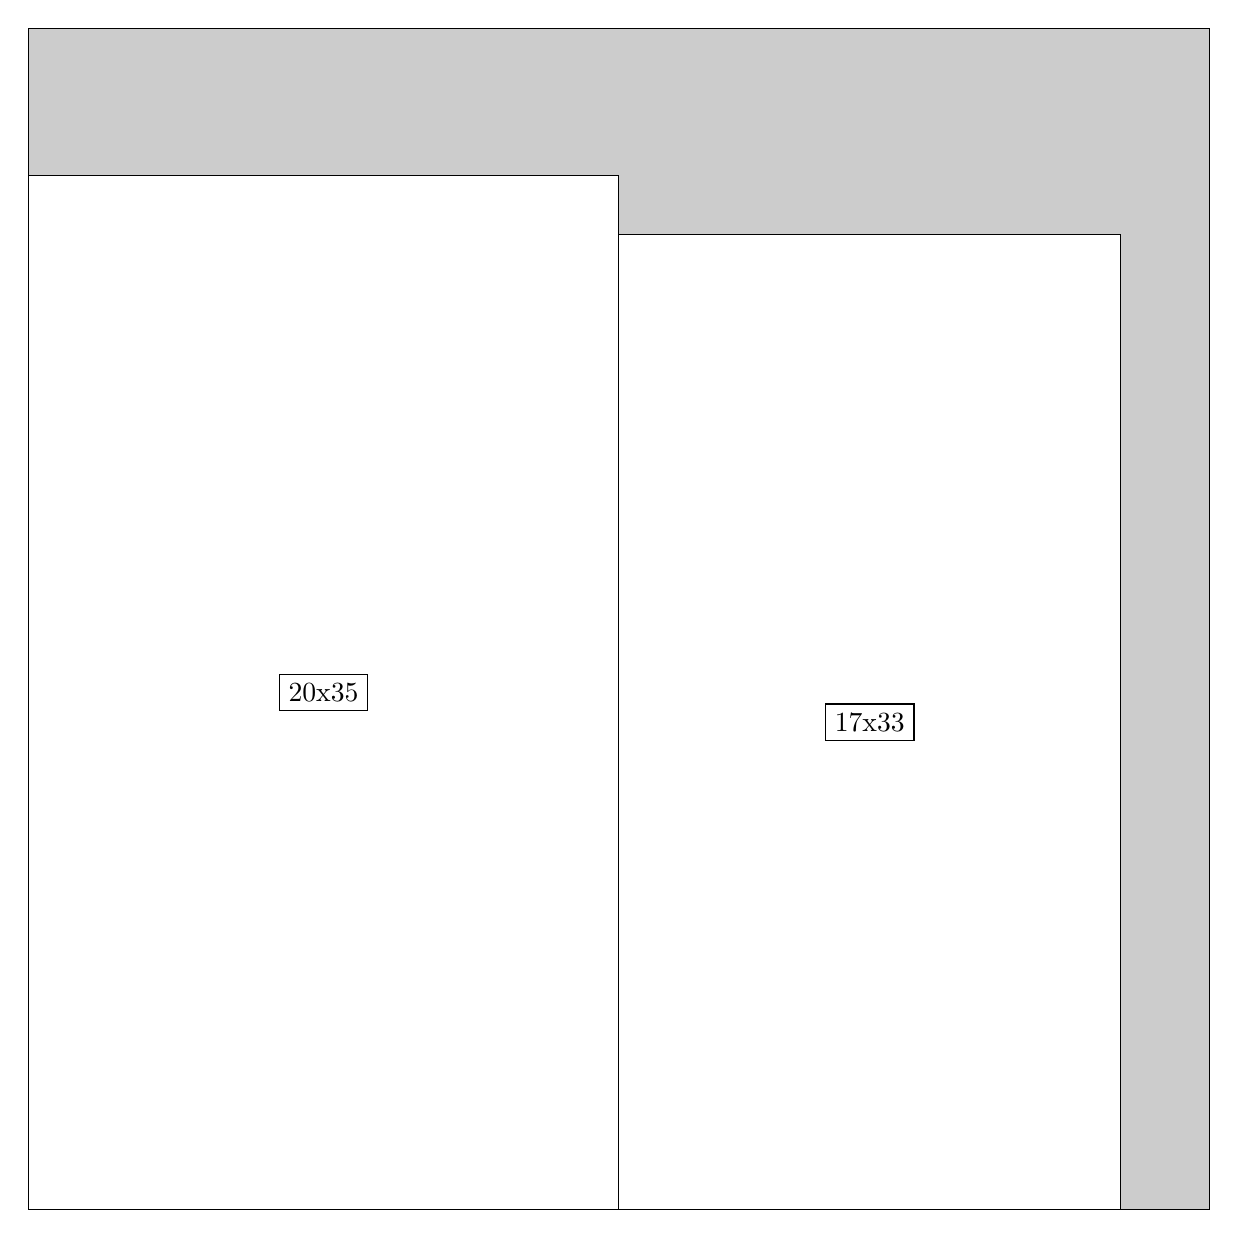
\begin{tikzpicture}[shorten >=1pt,scale=1.0,every node/.style={scale=1.0},->]
\tikzstyle{vertex}=[circle,fill=black!25,minimum size=14pt,inner sep=0pt]
\filldraw[fill=gray!40!white, draw=black] (0,0) rectangle (15.0,15.0);
\foreach \name/\x/\y/\w/\h in {20x35/0.0/0.0/7.5/13.125,17x33/7.5/0.0/6.375/12.375}
\filldraw[fill=white!40!white, draw=black] (\x,\y) rectangle node[draw] (\name) {\name} ++(\w,\h);
\end{tikzpicture}


w =20 , h =35 , x =0 , y =0 , v =700
\par
w =17 , h =33 , x =20 , y =0 , v =561
\par
\newpage


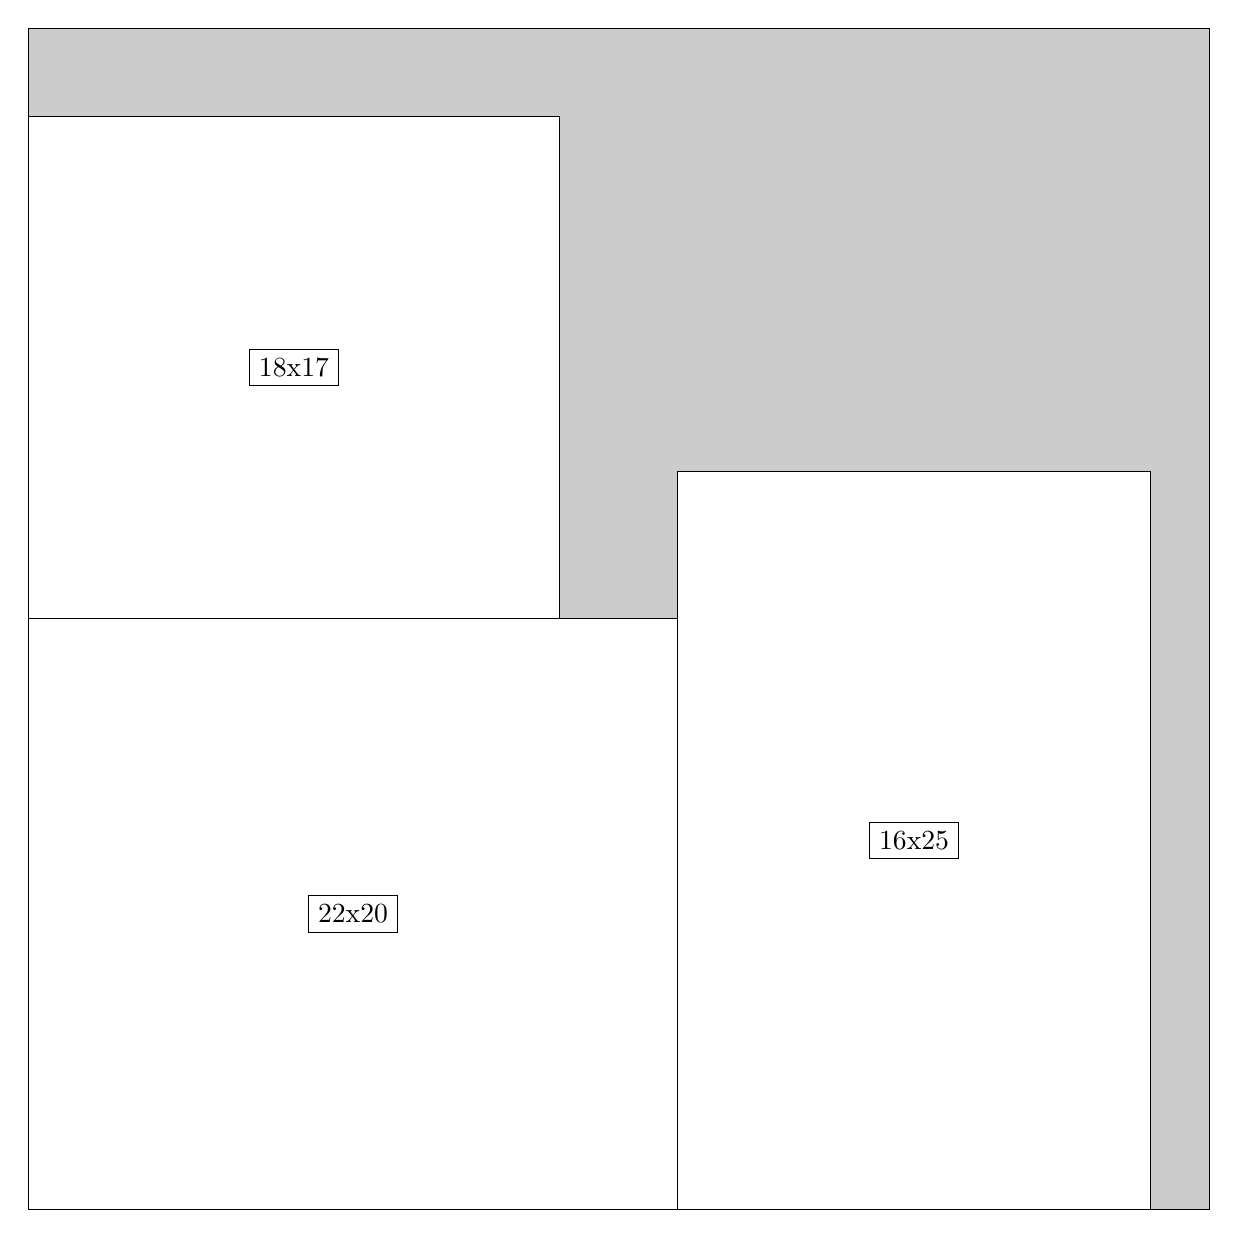
\begin{tikzpicture}[shorten >=1pt,scale=1.0,every node/.style={scale=1.0},->]
\tikzstyle{vertex}=[circle,fill=black!25,minimum size=14pt,inner sep=0pt]
\filldraw[fill=gray!40!white, draw=black] (0,0) rectangle (15.0,15.0);
\foreach \name/\x/\y/\w/\h in {22x20/0.0/0.0/8.25/7.5,16x25/8.25/0.0/6.0/9.375,18x17/0.0/7.5/6.75/6.375}
\filldraw[fill=white!40!white, draw=black] (\x,\y) rectangle node[draw] (\name) {\name} ++(\w,\h);
\end{tikzpicture}


w =22 , h =20 , x =0 , y =0 , v =440
\par
w =16 , h =25 , x =22 , y =0 , v =400
\par
w =18 , h =17 , x =0 , y =20 , v =306
\par
\newpage


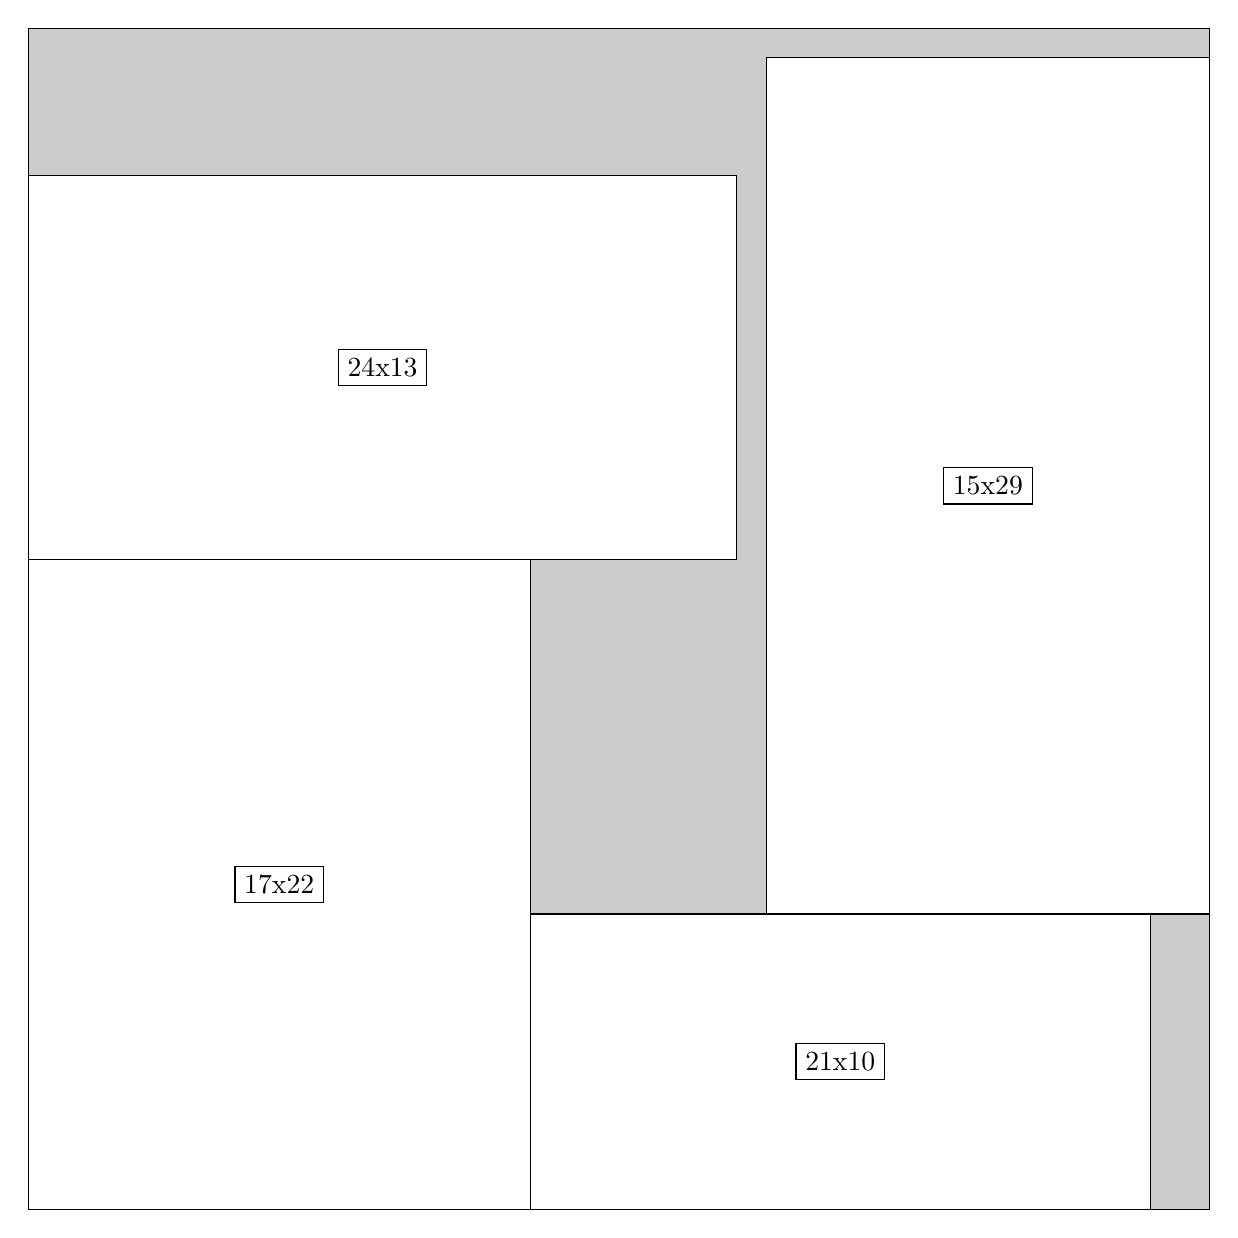
\begin{tikzpicture}[shorten >=1pt,scale=1.0,every node/.style={scale=1.0},->]
\tikzstyle{vertex}=[circle,fill=black!25,minimum size=14pt,inner sep=0pt]
\filldraw[fill=gray!40!white, draw=black] (0,0) rectangle (15.0,15.0);
\foreach \name/\x/\y/\w/\h in {17x22/0.0/0.0/6.375/8.25,24x13/0.0/8.25/9.0/4.875,21x10/6.375/0.0/7.875/3.75,15x29/9.375/3.75/5.625/10.875}
\filldraw[fill=white!40!white, draw=black] (\x,\y) rectangle node[draw] (\name) {\name} ++(\w,\h);
\end{tikzpicture}


w =17 , h =22 , x =0 , y =0 , v =374
\par
w =24 , h =13 , x =0 , y =22 , v =312
\par
w =21 , h =10 , x =17 , y =0 , v =210
\par
w =15 , h =29 , x =25 , y =10 , v =435
\par
\newpage


\end{document}